\documentclass{report}
\title{Thesis proposal: Understanding Outdoor Photometric Stereo}
\author{Yannick Hold-Geoffroy}
%\programme{Doctorat en g\'enie \'electrique}
%\annee{2015}


\date{\today}

%\usepackage{hyperref}
%\hypersetup{colorlinks,allcolors=ULlinkcolor}

%\frenchbsetup{%
%  CompactItemize=false,         % ne pas compacter les listes
%  ThinSpaceInFrenchNumbers=true % espace fine dans les nombres
%}


\usepackage[letterpaper, margin=1in]{geometry}
\usepackage[utf8]{inputenc}
\usepackage{times}
\usepackage{amsmath}
\usepackage{amssymb}
%\bibliographystyle{unsrtnat}
\usepackage[numbers,sort&compress]{natbib}
%\usepackage[numbers]{natbib}
%\usepackage{cite}   % sort citation numbers automatically
\usepackage{notoccite}
\usepackage{url}
\usepackage{graphicx}
\usepackage{rotating}
\usepackage{gensymb}
\usepackage{xcolor}
\usepackage{nicefrac}
%\usepackage{adjustbox}
%\usepackage{authblk}
% to control spacing in item lists
\usepackage[titletoc]{appendix}
\usepackage{enumitem}
\usepackage[pagebackref=false,breaklinks=true,colorlinks=true,linkcolor=black,bookmarks=true]{hyperref}
\usepackage{defs}
\usepackage{amsmath,esint}
\usepackage{titlesec}
\titleformat{\chapter}[display]
  {\normalfont\sffamily\huge\bfseries}
  %{\chaptertitlename\ \thechapter}{20pt}{\Huge}
  {\vspace{-5.5em}}{0pt}{\Large}
\titleformat{\section}
  {\vspace{-3em}\normalfont\sffamily\large\bfseries}
  {\large\thesection}{1em}{}

\linespread{1.5}


\begin{document}

%\frontmatter                    % pages liminaires

\maketitle
%\pagetitreonlyone                     % production des pages de titre

\tableofcontents

\hypersetup{colorlinks=true,linkcolor=blue}

% Commands
\newcommand*\B[1]{\mathbf{#1}}
\newcommand{\boldomega}{\boldsymbol \omega} % bold omega
\newcommand{\boldmu}{\boldsymbol \mu} % bold omega
\newcommand{\bolddelta}{\boldsymbol \delta} % bold delta

\newcommand\norm[1]{\left\lVert#1\right\rVert}

\newcommand\todo[1]{\textcolor{red}{TODO: #1}}

\graphicspath{{figures/}}

\chapter{Questions by Denis Laudenreau}

\section{Question 1}

\subsection{(a)}

Suppose q as the distance between the strip light and P along the x-axis.

\begin{equation}
E(r) = \frac{1}{\pi} \int_{\Omega} L(r,\omega)\cos(\theta) d\omega
\end{equation}
\begin{align*}
E(r) &= \frac{1}{\pi} \int_{-\arctan(\frac{\frac{H}{2}}{\sqrt{q^2+r^2}})}^{\arctan(\frac{\frac{H}{2}}{\sqrt{q^2+r^2}})} \int_{0}^{\arctan(\frac{w}{q})} L(r,\omega)\cos(\theta) \sin(\theta) d\theta d\phi \\
     &= 2 \cdot \arctan(\frac{\frac{H}{2}}{\sqrt{q^2+r^2}}) \cdot \int_{\arctan(\frac{q}{r-W/2})}^{\arctan(\frac{q}{r+W/2})} L(r,\omega)\cos(\theta) \sin(\theta) d\theta \\
     &= 2 \cdot \arctan(\frac{H}{2\sqrt{q^2+r^2}}) \cdot \left[ - \frac{1}{2} \cos^2(x) \right]_{\arctan(\frac{q}{r-W/2})}^{\arctan(\frac{q}{r+W/2})} \\
     &= 2 \cdot \arctan(\frac{H}{2\sqrt{q^2+r^2}}) \cdot \left[ - \frac{1}{2} \cos^2(\arctan(\frac{q}{r+W/2})) - - \frac{1}{2} \cos^2(\arctan(\frac{q}{r-W/2})) \right] \\
\end{align*}

\subsection{(b)}

As H gets bigger, the integral along the elevation axis gets closer toward $\pi$.

\subsection{(c)}



\section{Question 2}
\subsection{(a)}

$\Omega$
\begin{equation}
E(r) = \frac{1}{\pi} \int_{\Omega} L(r,\omega)\cos(\theta) d\omega
\end{equation}
\begin{align*}
E(r) &= \frac{1}{\pi} \int_{0}^{\arctan(\frac{h}{q})} \int_{0}^{\arctan(\frac{w}{q})} L(r,\omega)\cos(\theta) \sin(\theta) d\theta d\phi \\
     &= \arctan(\frac{h}{q}) \cdot \int_{0}^{\arctan(\frac{w}{q})} L(r,\omega)\cos(\theta) \sin(\theta) d\theta \\
     &= \arctan(\frac{h}{q}) \cdot \left[ - \frac{1}{2} \cos^2(x) \right]_{0}^{\arctan(\frac{w}{q})} \\
     &= \arctan(\frac{h}{q}) \cdot \left[ - \frac{1}{2} \cdot \cos^2(\arctan(\frac{w}{q})) - -\frac{1}{2} \right] \\
\end{align*}


\begin{equation}
E(r) = \frac{M}{2\pi} \sum_{i=1}^{n} \beta_i \cos(\alpha_i)
\end{equation}
\begin{align*}
E(r) = \frac{M}{2\pi} \left( \arctan(\frac{w}{q}) + \arctan(\frac{h}{q}) + \arctan(\frac{w}{q}) \cdot \cos(\arctan(\frac{h}{q})) + \arctan(\frac{w}{q}) \cdot \cos(\arctan(\frac{w}{q})) \right)
\end{align*}

\subsection{(b)}

\chapter{Questions by Philippe Giguère}

\section{Question 3}

\textbf{Impact of estimated light source error vs. estimated normal error (bias).}

The setup for this experiment is shown in fig.~\ref{q3:setup}. Three light sources forms an triangular pyramid with an equilateral triangle as its base. The problem states that its edge central angle is $r$.

\begin{figure}
  \centering
  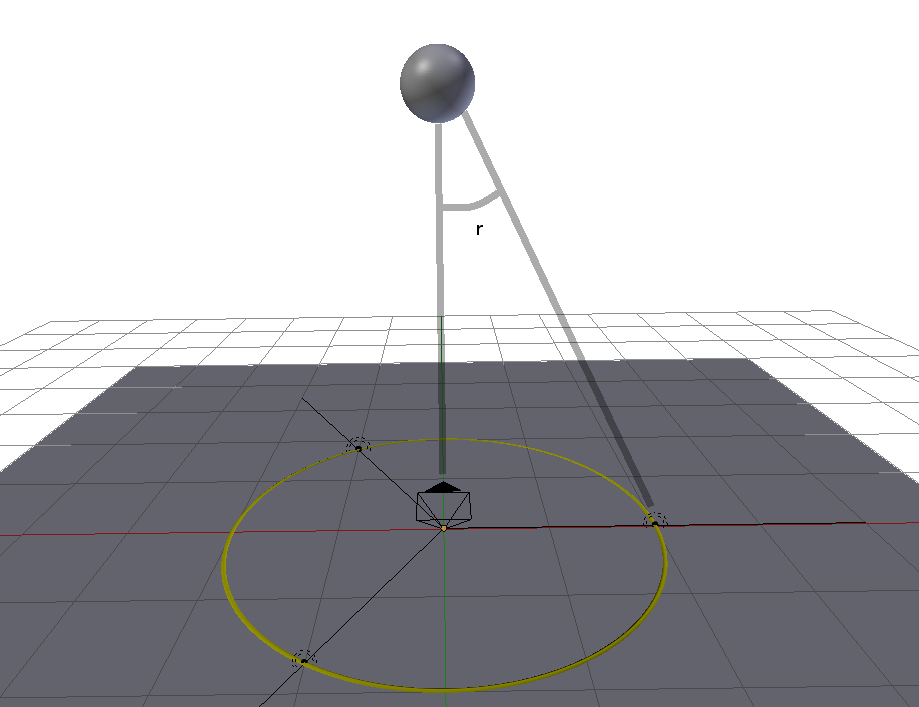
\includegraphics[width=0.9\linewidth]{q3_setup.png}
  \caption[Experiment setup]
   {Experiment setup.}
  \label{q3:setup}
\end{figure}

On this setup, each light, when lit, generate a row $\B{l}$ in the lighting matrix $\B{L}$ as such:
\begin{equation}
\B{l} =
\left[\begin{array}{c} \cos\!\left(\theta\right)\, \sin\!\left(r\right) \\ \sin\!\left(r\right)\, \sin\!\left(\theta\right) \\ \sqrt{ - {\cos\!\left(\theta\right)}^2\, {\sin\!\left(r\right)}^2 - {\sin\!\left(r\right)}^2\, {\sin\!\left(\theta\right)}^2 + 1} \end{array}\right]^T
\quad .
\end{equation}
The $x$ and $y$ components are directly the position on the plane, while the $z$ component is specified to make the light unit, so they are all the same intensity.

In the current setup, since the lights are on the vertex of an equilateral triangle, they are $120\degree$ apart on the $xy$-plane, so $\theta = \left[ 0\degree, 120\degree, 240\degree \right]$. This translates in the following lighting matrix:
\begin{equation}
\B{L} =
\left[\begin{array}{ccc} \sin\!\left(r\right) & 0 & \sqrt{1 - {\sin\!\left(r\right)}^2}\\ -\frac{\sin\!\left(r\right)}{2} & \frac{\sqrt{3}\, \sin\!\left(r\right)}{2} & \sqrt{1 - {\sin\!\left(r\right)}^2}\\ -\frac{\sin\!\left(r\right)}{2} & -\frac{\sqrt{3}\, \sin\!\left(r\right)}{2} & \sqrt{1 - {\sin\!\left(r\right)}^2} \end{array}\right]
\quad .
\end{equation}

Given the simple lambertian reflectance equation (supposing unit albedo), we can compute the pixel intensity of a camera pointed directly to a surface with normal $\B{n}$:
\begin{equation}
b = \B{L}\B{n}
\quad.
\end{equation}
Photometric Stereo is the inverse process, where the normals $\B{n} = \left[ n_x \; n_y \; n_z\right]^T$ are deduced from the lighting matrix $\B{L}$ and the pixel intensity $b$. This can be done by inverting the light matrix $\B{L}$, hence performing a least squares fit to the problem, as such:
\begin{equation}
\B{L}^{-1}\B{b} = \B{n} = 
\begin{bmatrix}
n_x \\
n_y \\
n_z 
\end{bmatrix}
\quad.
\end{equation}
We can see that, unless matrix $\B{L}$ is singular or affected by noise, we retrieve the three components of the normal $\B{n}$ directly.

But, instead of solving the usual equation, the problem suppose we have a systematic error $\epsilon_r$ in the measurement of $r$, making the noisy lighting matrix $\B{L}_\epsilon$ a bit different that the original matrix:
\begin{equation}
\B{L}_\epsilon = \left[\begin{array}{ccc} \sin\!\left(\epsilon_r + r\right) & 0 & \sqrt{1 - {\sin\!\left(\epsilon_r + r\right)}^2}\\ -\frac{\sin\!\left(\epsilon_r + r\right)}{2} & \frac{\sqrt{3}\, \sin\!\left(\epsilon_r + r\right)}{2} & \sqrt{1 - {\sin\!\left(\epsilon_r + r\right)}^2}\\ -\frac{\sin\!\left(\epsilon_r + r\right)}{2} & -\frac{\sqrt{3}\, \sin\!\left(\epsilon_r + r\right)}{2} & \sqrt{1 - {\sin\!\left(\epsilon_r + r\right)}^2} \end{array}\right]
\quad.
\end{equation}
Solving this problem gives us:
\begin{equation}
\B{L}_\epsilon^{-1}\B{b} = \B{n}_\epsilon = 
\left[\begin{array}{c} n_x \cdot \frac{\sin\!\left(r\right)}{\sin\!\left(\epsilon_r + r\right)}\\ n_y \cdot \frac{\sin\!\left(r\right)}{\sin\!\left(\epsilon_r + r\right)}\\ n_z \cdot \frac{\sqrt{1 - {\sin\!\left(r\right)}^2}}{\sqrt{1 - {\sin\!\left(\epsilon_r + r\right)}^2}} \end{array}\right]
\quad,
\end{equation}
where the normal components $n_x$, $n_y$ and $n_z$ are all multiplied by a non-unit factor due to the measurement error $\epsilon_r$. These factors are shown in fig.~\ref{q3:analytical}.

\begin{figure}
  \centering
  \begin{tabular}{cc}
  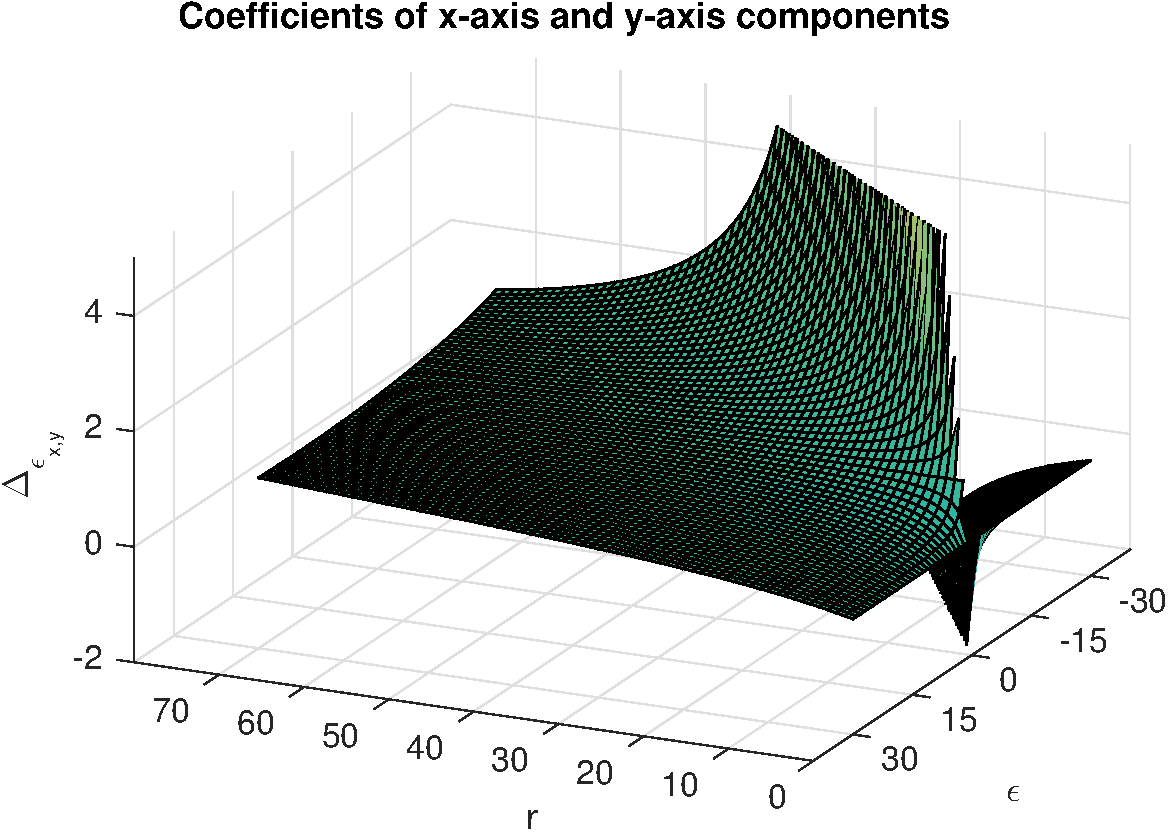
\includegraphics[width=0.45\linewidth]{q3_analytic_nx_ny.pdf} &
  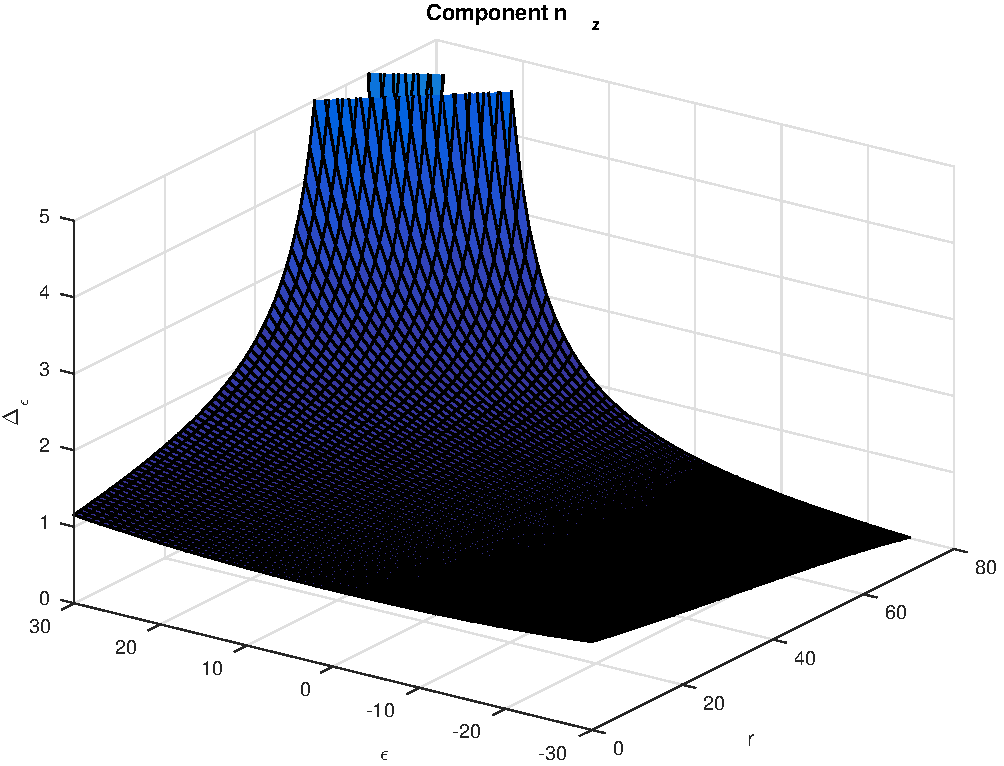
\includegraphics[width=0.45\linewidth]{q3_analytic_nz.pdf} \\
  (a) & (b)
  \end{tabular}
  \caption[Analytical normal component coefficients]
   {The theoretical factor $\Delta_\epsilon$ that multiplies each normal component (a) $n_x$, $n_y$ and (b) $n_z$ in the presence of a measure error $\epsilon_r$. When the factor is 1, no error is made on this component during the reconstruction (as it is the case when $\epsilon = 0$). A value less than 1 means the reconstructed normal component is smaller than the ground truth, while a value over 1 means a bigger component than the ground truth.}
  \label{q3:analytical}
\end{figure}

Until now, the noise impact was given analytically. If we try to actually perform a reconstruction on simulated data, there is something important to take into account. The conditioning of the matrix $\B{L}$ is very important, as it bounds the stability of the least-squares solution. This is even more related to this particular question because of the definition of the conditioning of the matrix $\kappa \left(\B{L}\right)$, as related by~\cite{ElGhaoui2002}:
\begin{equation}
\frac{ \| \B{L}_\epsilon ^{-1} - \B{L}^{-1} \| }{ \| \B{L}^{-1} \| }
\le \kappa\left(\B{L} \right) \frac{ \| \B{L}_\epsilon - \B{L}  \| }{ \| \B{L} \| }
\quad,
\end{equation}
where $\kappa \left(\B{L}\right) = \|\B{L}\| \cdot \|\B{L}^{-1}\|$. As~\cite{ElGhaoui2002} explains, ``the classical condition number $\kappa \left(\B{L}\right)$ is a measure of (relative) errors in the inverse of A when the latter is perturbed by an arbitrary, infinitesimally small matrix.''.

Two experiments are presented: first, in fig.~\ref{q3:exp1}, a surface normal $\B{n}$ is fixed while the lighting angle $r$ and measurement error $\epsilon_r$ varies. In the second experiment shown in fig~\ref{q3:exp2} and \ref{q3:exp2a}, a given lighting angle $r$ is fixed, while the surface normal $\B{n}$ and the measurement error $\epsilon_r$ varies. In both experiments, the angular error and reciprocal condition number $\frac{1}{\kappa\left(L\right)}$ are shown.

\begin{figure}
  \centering
  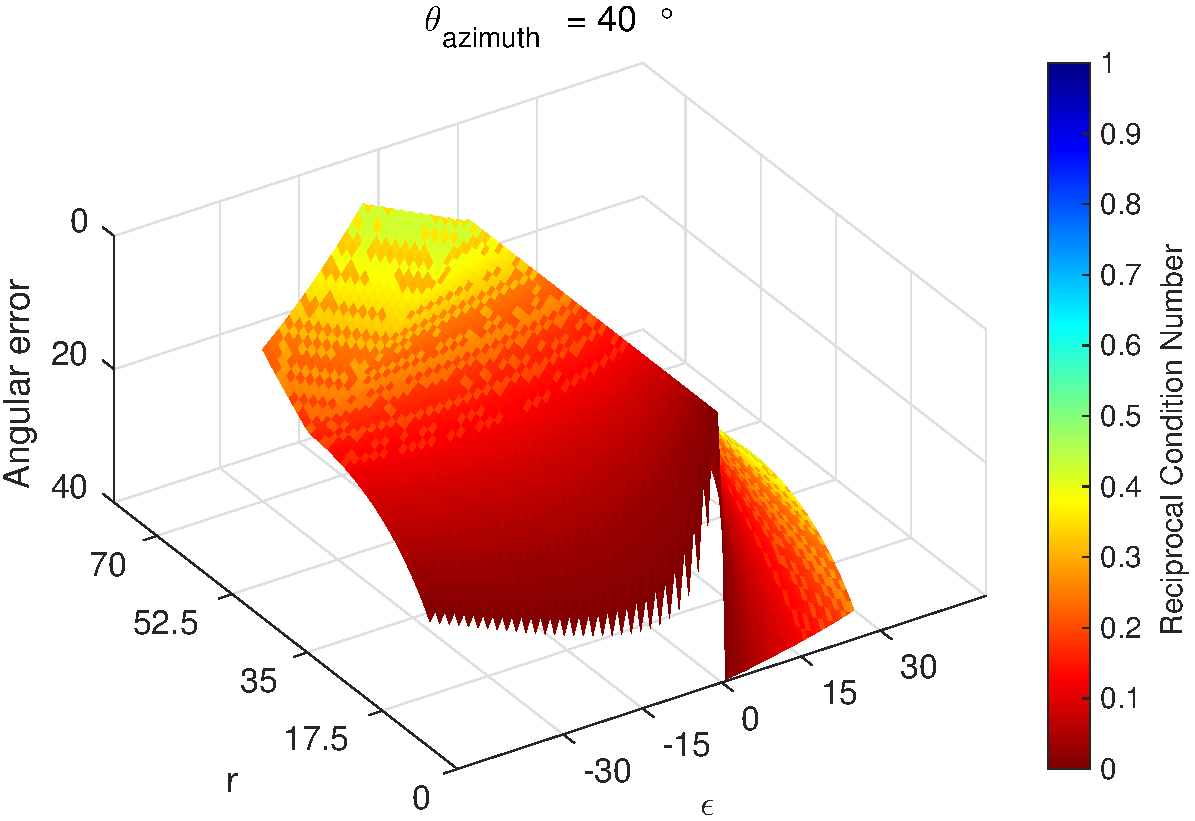
\includegraphics[width=0.45\linewidth]{q3_experiment_1_view_1.pdf}
  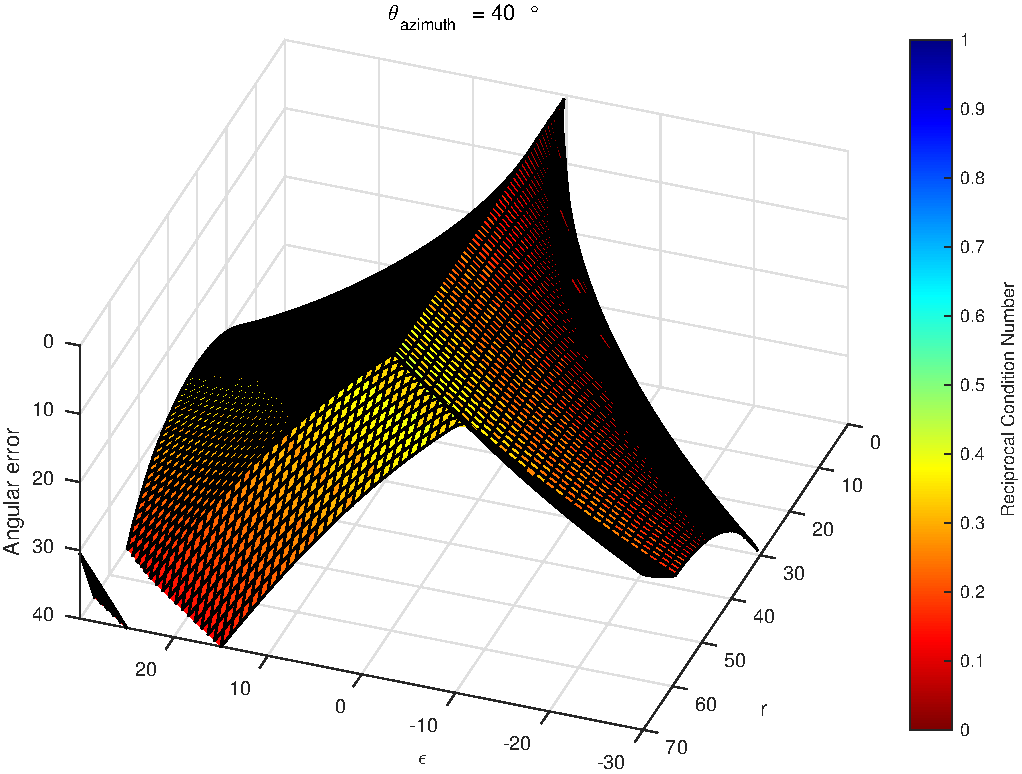
\includegraphics[width=0.45\linewidth]{q3_experiment_1_view_2.pdf}
  \caption[Experiment 1]
   {Angular error in degrees (z-axis) and reciprocal condition number (color) in function of $r \in \left[0, 70\right]$ (y-axis) and $\epsilon_r \in \left[-30, 30\right]$ (x-axis). The surface ground truth was set to 40\degree. \todo{make from normal/camera, not sphere} Both figures are two different point of views of the same function. Note how the region around $r = 30$ and $\epsilon = 10$ have a relatively good conditioning, but the result is much worse than regions with a lower measurement error $\epsilon$.}
  \label{q3:exp1}
\end{figure}

\begin{figure}
  \centering
  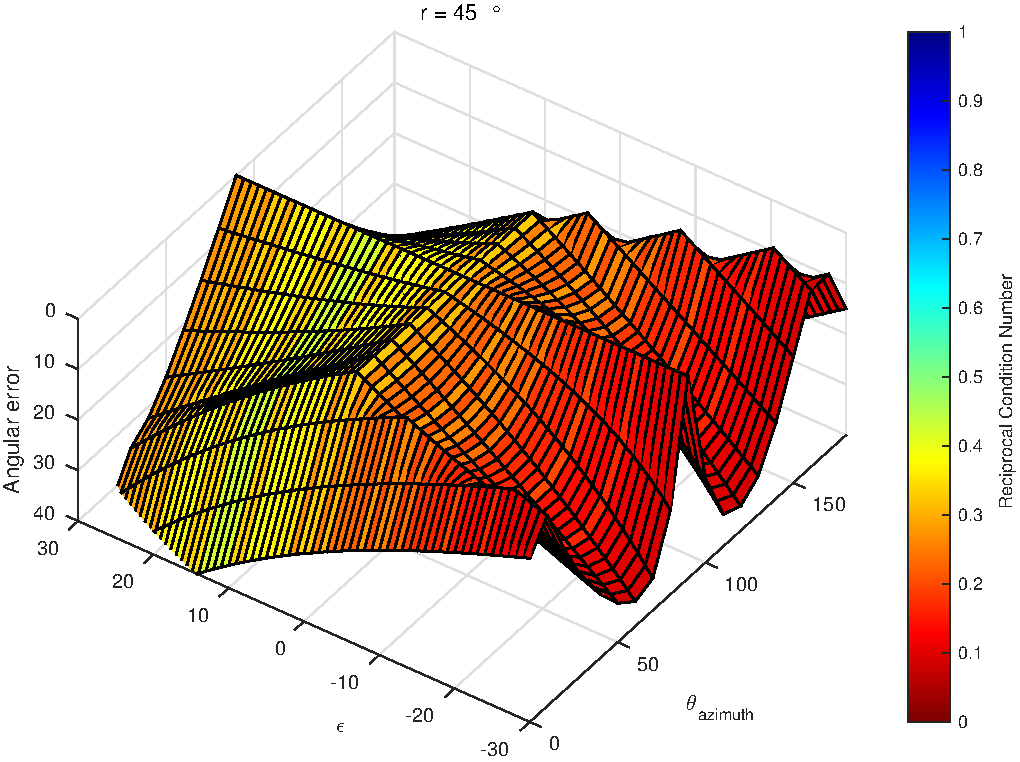
\includegraphics[width=0.45\linewidth]{q3_experiment_2_view_1.pdf}
  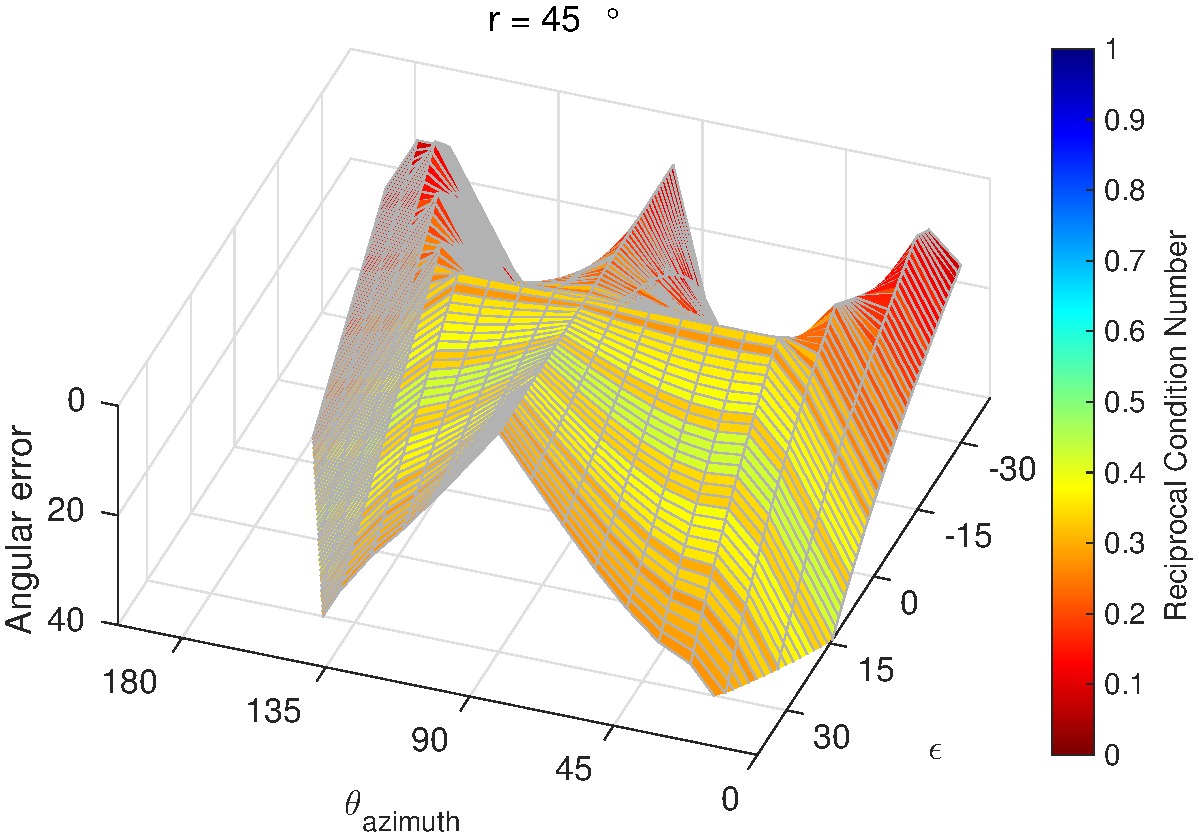
\includegraphics[width=0.45\linewidth]{q3_experiment_2_view_2.pdf}
  \caption[Experiment 2]
   {Angular error in degrees (z-axis) and reciprocal condition number (color) in function of $\theta_{\mathrm{azimuth}} \in \left[0, 180\right]$ (y-axis) and $r \in \left[0, 70\right]$ (x-axis). Both figures are two different point of views of the same function. Note how the region around $r = 30$ and $\epsilon = 10$ have a relatively good conditioning, but the result is much worse than regions with a lower measurement error $\epsilon$.}
  \label{q3:exp2}
\end{figure}

\begin{figure}
  \centering
  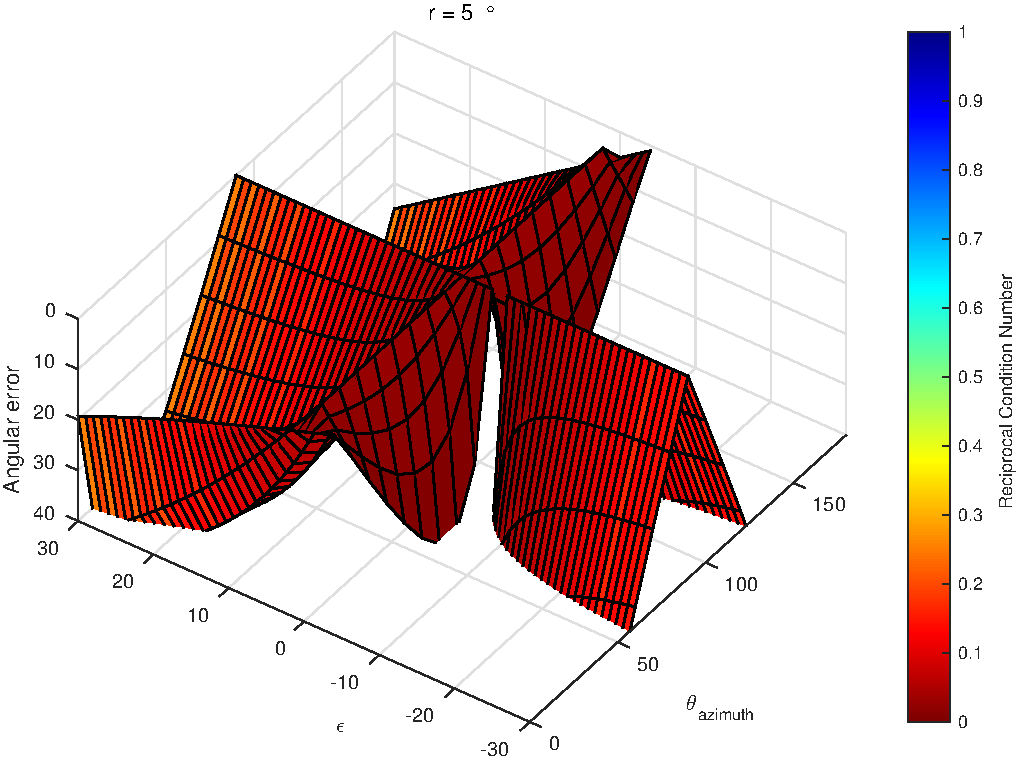
\includegraphics[width=0.45\linewidth]{q3_experiment_2a_view_1.pdf}
  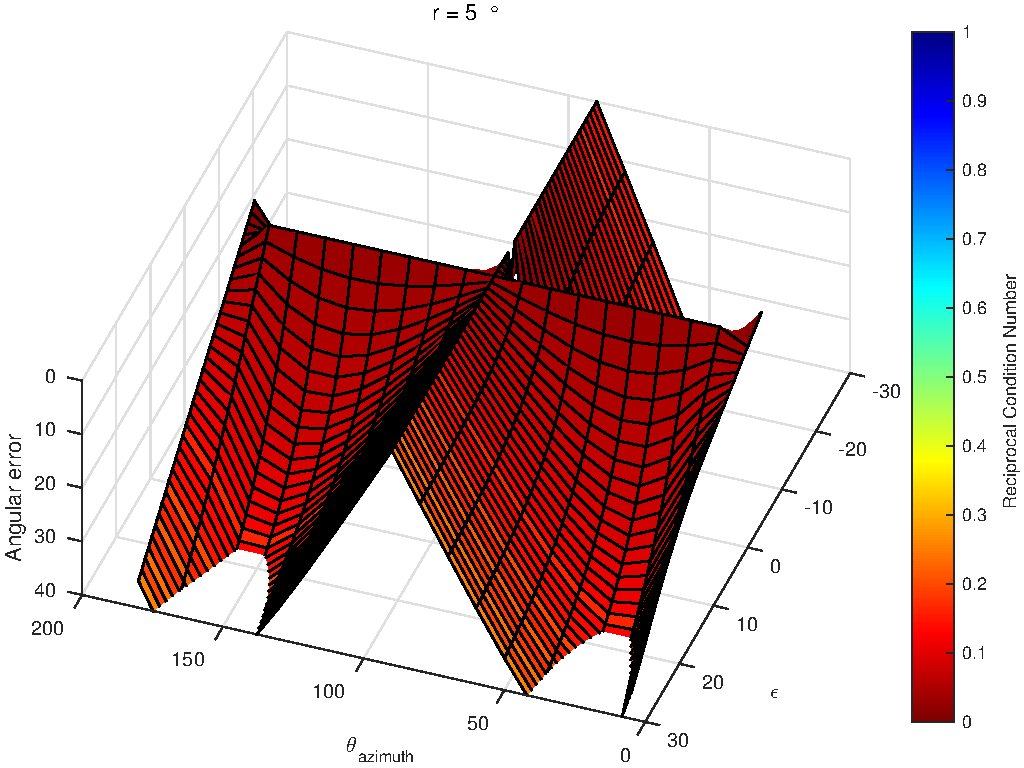
\includegraphics[width=0.45\linewidth]{q3_experiment_2a_view_2.pdf}
  \caption[Experiment 2 on extreme values]
   {Experiment setup.}
  \label{q3:exp2a}
\end{figure}

It is interesting to note [...].

\section{Question 4}

\chapter{Questions by Paulo Gotardo}

\section{Question 5}
\subsection{(a)}
\textbf{Let $\B{A} \in \mathbb{R}^{m \times n}$, with $m \gg n$. Show how the eigenvalues and (unit) eigenvectors of $\B{AA}^T$ can be obtained from the eigen decomposition of the smaller matrix $\B{A}^T\B{A}$.}

By the definition of the Singular Value Decomposition (SVD), any matrix real $A$ can be factored such as
\begin{equation}
\B{A} = \B{U \Sigma V}^T \quad.
\end{equation}
Matrices $\B{U}$, $\B{\Sigma}$ and $\B{V}$ are closely related to the eigen decomposition. First, $\Sigma$ is a diagonal matrix yielding the singular values of $A$, which are the square roots of the eigenvalues of both $\B{AA}^T$ and $\B{A}^T\B{A}$. Second, the columns of $\B{U}$ and $\B{V}$ are, by definition, the eigenvectors of $\B{AA}^T$ and $\B{A}^T\B{A}$, respectively. We can convince ourselves of both with these relations:
\begin{align*}
\B{AA}^T           &= \B{V\Sigma}^T\B{U}^T \; \B{U\Sigma V}^T
                        &&= \B{V\Sigma}^T\B{IU\Sigma V}^T 
                        &&&= \B{V\Sigma}^T\B{\Sigma V}^T \quad,\\
\B{A}^T\B{A}  &= \B{U\Sigma V}^T \; \B{V\Sigma}^T\B{U}^T
                        &&= \B{U\Sigma V}^T \; \B{V\Sigma}^T\B{U}^T
                        &&&= \B{U\Sigma}\B{\Sigma}^T\B{U}^T \quad.
\end{align*}
As the columns of $\B{U}$ and $\B{V}$ are a orthonormal basis (as they hold the eigenvectors), both $\B{U}^T\B{U}^T$ and $\B{V}^T\B{V}$ gives the identity matrix $\B{I}$ as result.

Two relationships are sought in the question: the eigenvalues and eigenvectors of both pre and post multiplication by the transpose. First, the relationship between the eigenvalues of $\B{A}^T\B{A}$ and $\B{AA}^T$ is pretty simple: they are the same. On the other hand, both their eigenvectors is only related through $\B{A}$:
\begin{align*}
\B{A}  &= \B{U \Sigma V}^T \\
\B{AV} &= \B{U \Sigma V}^T \B{V} = \B{U \Sigma I} \\
\B{AV\Sigma}^\dagger &= \B{U \Sigma \Sigma}^\dagger = \B{U} \quad,
\end{align*}
where $\B{\Sigma}^\dagger$ is the pseudoinverse of $\B{\Sigma}$. This $\B{\Sigma}^\dagger$ is used as a normalization factor for the $\B{AV}$ matrix; normalizing each column of $\B{AV}$ would produce the same result.

This relation will provide as many eigenvectors as there are linearly independent vectors of $\B{AA}^T$. Since $m \gg n$, this means that at most $n$ eigenvectors of $\B{AA}^T$ will be found. The rest of the resulting matrix will contain only zeros. The vectors that are missing span the null space of $\B{A}^T$ (and $\B{AA}^T$).

\subsection{(b)}



\subsection{(c)}
\section{Question 6}

Temporally-multiplexed Photometric Stereo employs captures at different times yielding different lighting directions. This means that each row of the lighting matrix $\B{L}$ are taken at a different time, when the scene's lighting condition changed. Contrarily, as \cite{Fyffe2011} puts it, ``In Spectrally-multiplexed photometric stereo, a scene is illuminated by multiple spectrally distinct light sources, and photographed by a camera system configured to capture multiple spectrally distinct color channels.'' In their work, they propose to divide the light spectrum in two using the Dolby\textsuperscript{\textregistered} dichroic filters, both having some non-overlapping red, green, and blue in their response spectrum.

Typically, PS is performed on pixel intensities, also called the luminance $y_i$ of a pixel $i$. This luminance can be expressed as a weighted sum of each pixel components, red $r_i$, green $g_i$ and blue $b_i$. The coefficients of the weighted sum depends on the colorspace used and on the measure (e.g.\ energy or perception). The two main luminance coefficients are based on the CIE 1931 colorspace, $y_i = 0.2126r_i + 0.7152g_i + 0.0722b_i$ and its perceptually based counterpart, $y_i = 0.299r_i + 0.587g_i + 0.114b_i$. This conversion to luminance can be problematic when analyzing natural illumination, though. Most of the energy in natural illumination, aside from the sun, is contained in the blue channel (as the sky is blue). However, this particular channel gets weighted down the most, as the blue channel coefficient is the lowest ($0.0722$ or $0.114$ in the earlier examples), making its impact on luminance much less than the other channels. To mitigate this issue, sophisticated channel fusion techniques have been proposed (e.g.\ \cite{jung-cvpr-15}), but this approach is clearly not a panacea to the problem.

This is where temporally-multiplexed outdoor photometric stereo can benefit from the color spectrum. To prevent the loss of information of merging the color channels together, \cite{johnson-cvpr-11} propose to take each color channel as different captures, yielding different light sources. They argue that the information contained in every color channel of an image lit by natural illumination is enough in most cases to bring new constraints to the PS problem, helping the reconstruction. Hence, every picture taken could fill 3 rows of the $\B{L}$ matrix, one row per channel. This works because natural illumination is complex and may yield sensibly different lighting vectors for each channel. Cloud occlusion could notably shift the color of the sun \todo{untested}.

There is a reason why \cite{Fyffe2011} employed such a complex apparatus using dichroic filters, though, instead of simply using the three channels of a common camera. If the albedo of the target object is mostly red, for example, it will have an almost null pixel intensity in the green and blue channels, potentially boosting the noise of the latter channels. \todo{bad example} Considering purely red, green or blue lights sometimes becomes a two-sources problem if a source a particular channel is in shadow. Furthermore, the algorithm provided by \cite{johnson-cvpr-11} suppose a constant albedo over the whole surface.
%\cite{MacDonald-2007}.

It is nevertheless an interesting idea worth exploring when performing further analysis on photometric stereo.

\section{Question 7}

Such an algorithm is presented in~\cite{Granados2010a}. The goal is to estimate, as best as possible, the irradiance $X_i$ of each pixel $i$. This is done by merging images of different exposure $j$ together. Basically, this algorithm is as follows:
\begin{enumerate}
  \item{Acquire dark frames for all exposures values $e_j$;}
  \item{Assume constant variances $\hat{\sigma}_{X_j}^2{}^{(0)}$}
  \item{Compute the maximum likelihood estimate $\hat{\mu}_X^{(j)}$ for each pixel irradiance taking into account $\hat{\sigma}_{X_j}^2{}^{(j-1)}$;}
  \item{Estimate the pixel variances $\hat{\sigma}_{X_j}^2{}^{(j)}$ taking into account $\hat{\mu}^{(j-1)}$;}
  \item{Repeat the two previous steps until convergence;}
  \item{Smooth the final maximum likelihood estimate $\hat{\mu}_X$ according to the pixel variances $\hat{\sigma}_{X_j}^2$}
\end{enumerate}

The optimal weighting function $w_{\mathrm{opt}}\left(v_j\right)$ of every pixel $v_j$ is the reciprocal of the pixel variances $\frac{1}{\hat{\sigma}_{X_j}^2}$.

This algorithm is based on the idea that the pixel $i$ on an image of given exposure $j$ has an irradiance $X_{ij}$ related to the according to the image taken $V_j$ dark frame $B_j$, the exposure time $t_j$ and the camera gains $g$ (global) and $a$ (non-uniform, pixel-dependent) as such:
\begin{equation}
\label{q7:eqirr}
X_{ij} \approx \frac{V_{ij} - B_{ij}}{t_j \cdot g \cdot a}
\quad.
\end{equation}

Two types of noise is taken into account in this analysis: the thermal noise and spatial noise. In the first category fall the Photon Shot Noise, accounting the uncertainty of photons arrival and amounting to $\sqrt{\frac{X}{t_j}}$, the Dark Current Shot Noise, accounting for electron movement not caused by incoming photons, and the readout noise, explaining the noise and imprecision in the electronic circuit producing the output digital values. The second category, spatial noise, regroup Photo-Response Non-Uniformity, accounting for variability in gain over the various pixels, and the Dark Current Non-Uniformity, accounting for dark current variability across the sensor surface due to temperature differences.

The output digital value $V$ of a pixel $i$ on image $j$ is related to the irradiance it received $X_{ij}$ by the exposure time $t_j$, the dark current $D_i$, the readout noise $N_R$ and sensor gains $g$ and $a_i$ as such:
\begin{equation}
V_{ij} = \left[ g \cdot \left( t_j \left( a_i X_i + D_i \right ) + N_R\right) \right] \quad,
\end{equation}
where $\left[ \cdot \right]$ is the rounding operator. The variance of this pixel output value is
\begin{equation}
\label{q7:noisevariance}
\sigma_{V_{ij}}^2 = g^2 \sigma_{E_{ij}}^2 + \sigma_R^2
\quad,
\end{equation}
where $\sigma_{E_{ij}}^2$ is the Photon Shot Noise and Dark Current Shot Noise combined, and $\sigma_R^2$ the readout noise, including the quantization error.

Plugging the variance of pixel output values~\eqref{q7:noisevariance} into the irradiance equation \eqref{q7:eqirr}, we get:
\begin{equation}
\sigma_{X_{ij}}^2 = \frac{\sigma_{V_{ij}}^2 + \sigma_{B_{ij}}^2}{t_j^2 g^2 a_i^2} \quad.
\end{equation}

This analyze takes into account a single image. When merging the images together to form a HDR restoration, the variance due to noise becomes:
\begin{equation}
\sigma_{\mu_{X_{ij}}}^2 = \frac{1}{\sum_{j \in S_i} \frac{t_j^2 g^2 a_i^2}{g^2 t_j \left( a_i \mu_{X_i} + 2 \mu_{D_i} \right) + 2 \sigma_R^2}} \quad,
\end{equation}
when taking into account the set of images $S_i$ at pixel $i$.

\chapter{Questions by Jean-François Lalonde}

\section{Question 8}
\subsection{(a)}
\textbf{Given a known lighting environment map $\B{L}$ (e.g.\ in latitude-longitude representation), explain how SH coefficients $s$ can be estimated from $\B{L}$.}

Each SH coefficients $s$ is linked to a basis function of order $n$ and mode $m$ defined over the sphere. Because these basis functions are orthogonal, the coefficients are computed by projecting the environment map $\B{L}$ on the according basis function, called $Y_n^m$:
\begin{equation}
s_n^m = \oiint\limits_{\Omega} \B{L}\left(\B{\omega} \right) Y_n^m \left( \B{\omega} \right) \mathrm{d} \B{\omega}   \quad.
\end{equation}
This formulation produces the least-squares fit of the basis functions over the environment map $\B{L}$.

In the discrete case, just like the environment map $\B{L}$, these functions can be represented in latitude-longitude representation. This allows the projection to be performed as the summation of its pixelwise multiplication with the environment map $\B{L}$:
\begin{equation}
s_n^m = \sum_{v=0}^{h} \sum_{u=0}^{w} \B{L}_{u,v} Y_n^m\left(u, v\right) \omega_{u,v}^2 \quad,
\end{equation}
for an environment map $\B{L}$ of width $w$ and height $h$. The solid angle subtended by pixel $u,v$, called $\omega_{u,v}$, is required to weight accordingly each pixel of both maps. Because of the latitude-longitude representation, each pixel covers a different surface area over the sphere. Without this solid angle weighting, pixels near the top and bottom edge of the environment map are more important, resulting in a brighter  [...].


\begin{equation}
s_3^2 = \sum \underbrace{\begin{minipage}{84pt}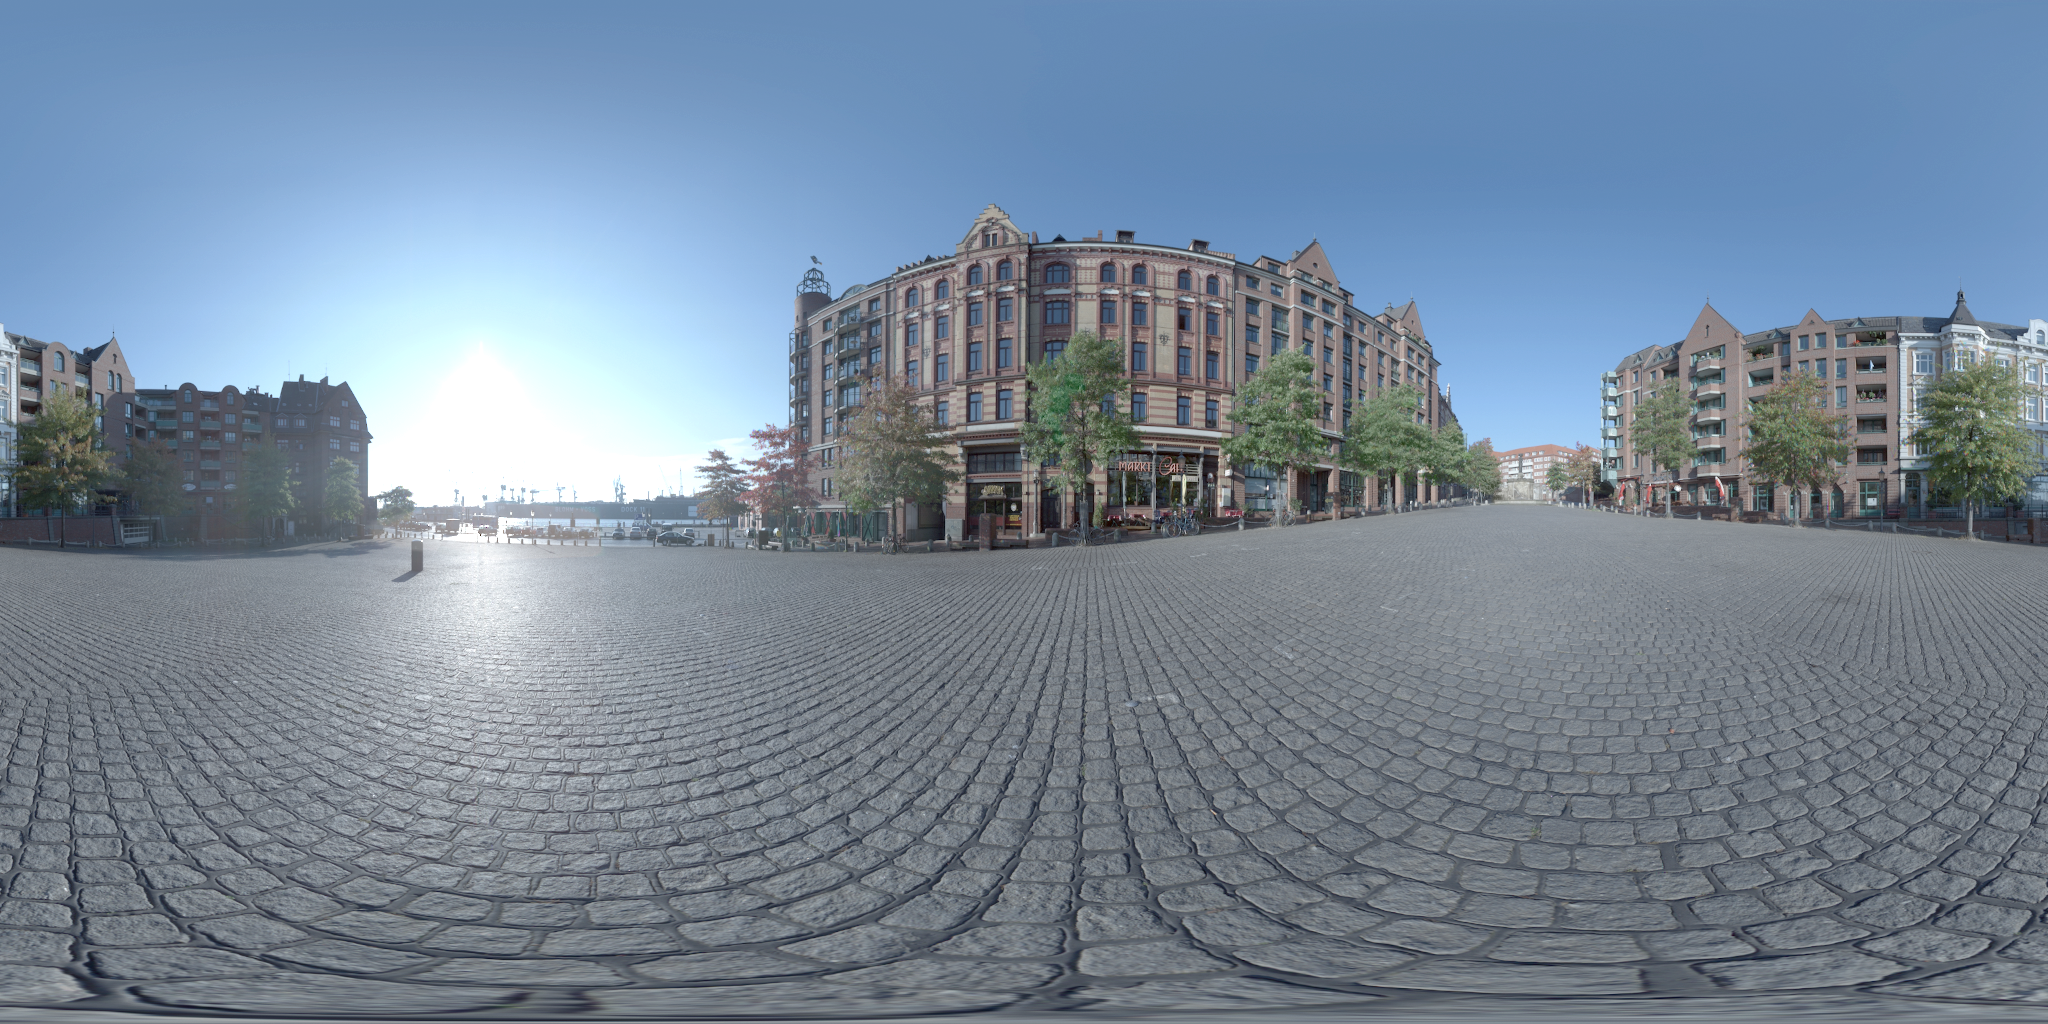
\includegraphics[height=42pt,width=84pt]{q8_envmap.png}\end{minipage}}_{\text{Environment map}} \cdot
\left(
\underbrace{\begin{minipage}{84pt}
\includegraphics[height=42pt,width=84pt]{q8_basis_3_2_real.png}\end{minipage}}_{\mathrm{Re}(Y_3^2)} + 
\underbrace{\begin{minipage}{84pt}
\includegraphics[height=42pt,width=84pt]{q8_basis_3_2_imag.png}\end{minipage} \; i}_{\mathrm{Im}(Y_3^2)}
\right)
\cdot
\left(
\underbrace{\begin{minipage}{84pt}
\includegraphics[height=42pt,width=84pt]{q8_solidangle.png}\end{minipage}}_{\text{Solid Angle}}
\right)^3
\quad.
\end{equation}


\begin{figure}[hb]
  \centering
  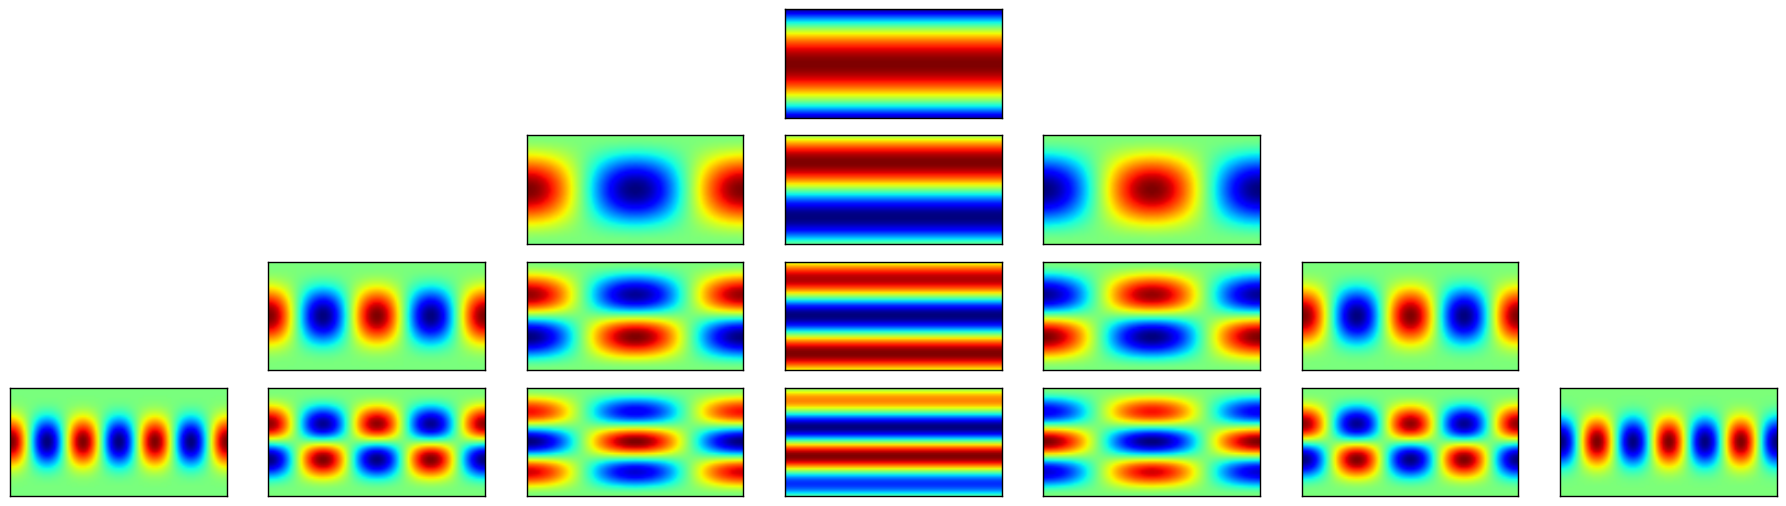
\includegraphics[width=0.45\linewidth]{q8_a_pyramid_real.png}
  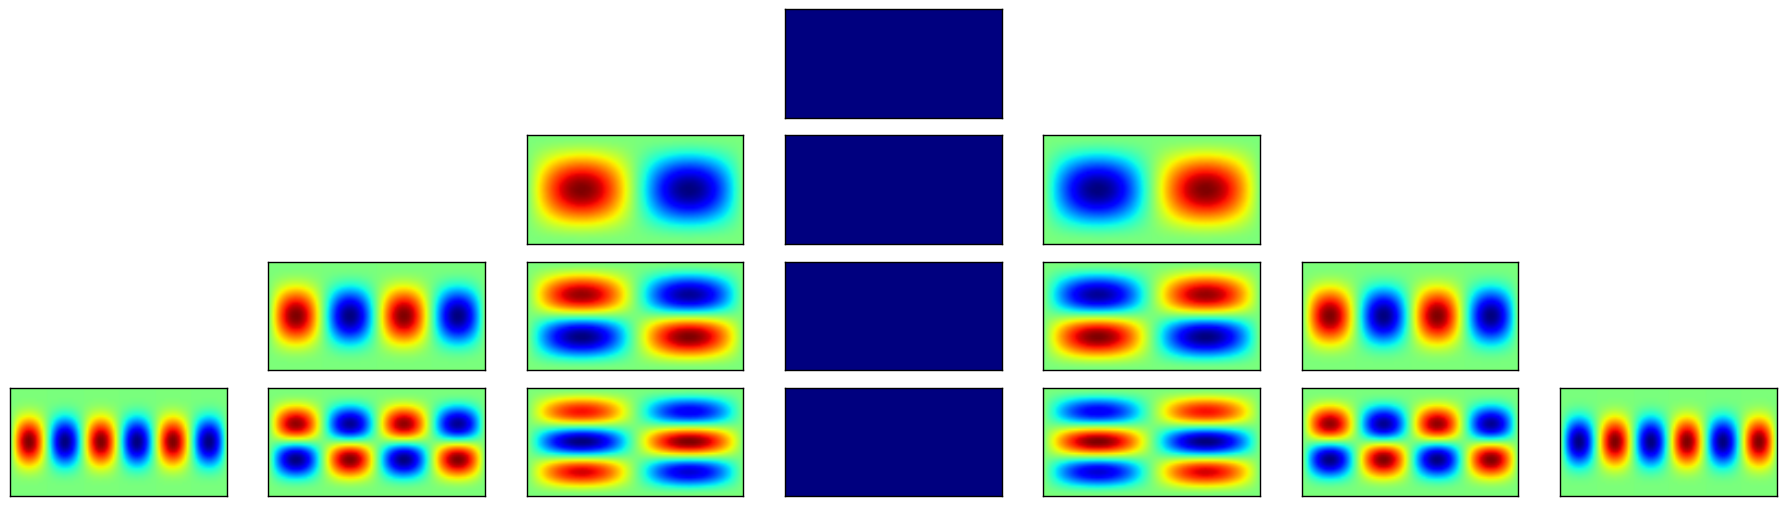
\includegraphics[width=0.45\linewidth]{q8_a_pyramid_imag.png}
  \caption[Sample Spherical Harmonics]
   {Basis of degrees 0-3 of Spherical Harmonics}
\end{figure}

%Just like the Fourier transform, Spherical Harmonics is a transform using a principal root of unity as its kernel. Having a kernel based on a principal root of unity over the function's domain confers a plethora of interesting attributes. One of which is that the functions generated form an orthonormal basis spanning the whole domain, called a complete orthonormal system.

This pixelwise multiplication works because the SH basis forms an orthonormal system. Projecting something on an orthonormal basis can be called a dot product, because it yields the same properties. Thus, this relation holds \emph{iif} $f(x)$ and $g(x)$ are orthogonal over period $p$:
\begin{equation}
f \cdot g=\int_{-p}^p f(x)g(x)\,dx\ \quad,
\end{equation}
explaining why discrete transforms in general (SH, Fourier, Z, etc.) work using a single per-element multiplication.
\todo{least squares?}

%Computing a coefficient $s$ of a given order $n$ and mode $m$ of spherical harmonic is be done by projecting the base $Y_n^m$ on the environment map $\B{L}$. Given a latitude-longitude representation,

\subsection{(b)}

The signal reconstructed from the Spherical Harmonic transform (using all the SH coefficients $s$ present in the signal) is proved to be exactly the same than the original signal. Negative values reconstructed from a strictly positive input cannot happen when performing the whole transform. One problem, though, is that computing the whole Spherical Harmonic transform can be excessively long on medium to big input signals. People often take a low-frequency approximation of their signal by computing only the first SH coefficients $s$, which, when reconstructed, may bear some errors potentially making some values becoming negative.

In such case, the one and only way to reconstruct strictly positive (or null) lighting $\bar{\B{L}}_{\mathbf{nonneg}}$ is by thresholding the reconstruction result $\bar{\B{L}}$:
\begin{equation}
\bar{\B{L}}_{\mathbf{nonneg}} = \max\left( 0, \bar{\B{L}} \right) \quad.
\end{equation}

That being said, as~\cite{Sloan2008} \todo{others?} relate, the amount of negative lighting can be greatly reduced in two ways:
\begin{enumerate}
  \item{Performing windowing on the signal;}
  \item{Performing the projection using an optimization with regularization to enforce positive light.}
\end{enumerate}

The first involves convolving the input signal with a window such as Hanning or Lanczos to limit the ringing effect of projecting onto a base-a major cause of negative reconstruction values-, called the Gibbs phenomenon. By the convolution theorem, performing an element-wise multiplication in the frequency domain after the projection would produce an identical result in a less expensive way, in terms of computational effort. This technique works by removing the higher frequencies of a signal before projecting it, mitigating some of the impact of sharp variations on the projection. This is analogous to the low-pass filter applied to an image before downscaling it\todo{?}.

The second option changes the projection step to add a regularization:
\begin{equation}
\arg \min_s \int\left( \bar{\B{L}}(\omega) - \B{L}(\omega)\right)^2 \mathrm{d}\omega + \lambda \int \left(\Delta \bar{\B{L}}(\omega)\right)^2 \mathrm{d}\omega
\end{equation}

\subsection{(c)}
HH paper
\subsection{(d)}
Stupid SH tricks
\section{Question 9}

{\small
\bibliographystyle{acm}
\bibliography{library}
}

\end{document}
